%--------------------
% Packages
% -------------------
\documentclass[12pt,a4paper]{article}
% \usepackage[a4paper, left=15mm, right=15mm, top=15mm, bottom=15mm]{geometry}
\usepackage[utf8x]{inputenc}
\usepackage[T1]{fontenc}
%\usepackage{gentium}
\usepackage{mathptmx} % Use Times Font
% \usepackage[siunitx]{circuitikz} % for circuit schematics
\usepackage{siunitx}
\usepackage{amsmath} % for the equation* environment
\usepackage{graphicx}
\usepackage{pgfplots}
\pgfplotsset{compat=1.14}
\usepackage{float}

\usepackage{graphicx} % Required for including pictures % clashes with circuitikz
% \usepackage[swedish]{babel} % Swedish translations
\usepackage[pdftex,linkcolor=black,pdfborder={0 0 0}]{hyperref} % Format links for pdf
\usepackage{calc} % To reset the counter in the document after title page
\usepackage{enumitem} % Includes lists

\frenchspacing % No double spacing between sentences
\linespread{1.2} % Set linespace
\usepackage[a4paper, lmargin=0.08\paperwidth, rmargin=0.08\paperwidth, tmargin=0.08\paperheight, bmargin=0.08\paperheight]{geometry} %margins
%\usepackage{parskip}
% \usepackage[all]{nowidow} % Tries to remove widows
\usepackage[protrusion=true,expansion=true]{microtype} % Improves typography, load after fontpackage is selected

\usepackage[inkscapelatex=false]{svg}
\graphicspath{ {./media/} }

% \pagecolor{black}
% \color{white}

\usepackage{setspace}


%-----------------------
% Set pdf information and add title, fill in the fields
%-----------------------
\hypersetup{ 	
pdfsubject = {},
pdftitle = {ee5311-2025-ee24s053-pwc-report-tut5},
pdfauthor = {Karthik B K <ee24s053@smail.iitm.ac.in>}
}

%-----------------------
% Begin document
%-----------------------
\begin{document}

\title{EE5311 \\ Report of Practical Work Conducted for Tutorial 06 (b)}
\author{Karthik B K ee24s053}
\maketitle

\section{Experiment A}
\subsection{Calculations}
\noindent We use the layouts from simulation 6a to construct an 8-bit ripple carry adder.
\subsection{Layouts}
\noindent We draw the following layout using \emph{klayout}.
\begin{center}
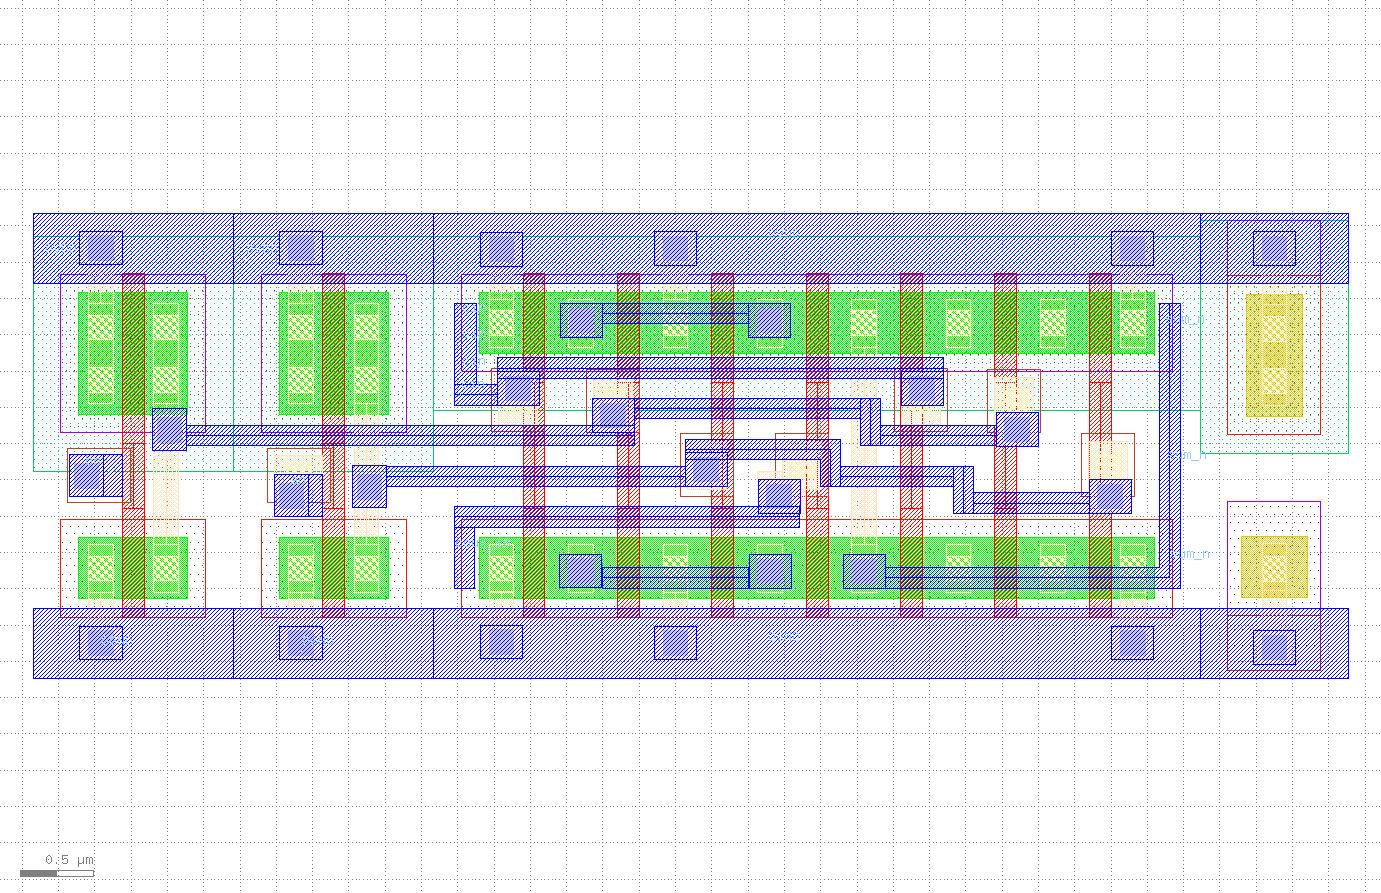
\includegraphics[width=0.99\linewidth]{tut6/rca/sum/sum.gds.png} \\
Fig 1: Layout of the 8-bit Ripple Carry Adder
\end{center}

\noindent All the above layouts are DRC and LVS clean.

\subsection{Measurements}
\noindent We perform a transient simulation with the setup both before and after layout extraction for the inverter and obtain the following plots.
\begin{center}
\begin{tabular}{cc}
     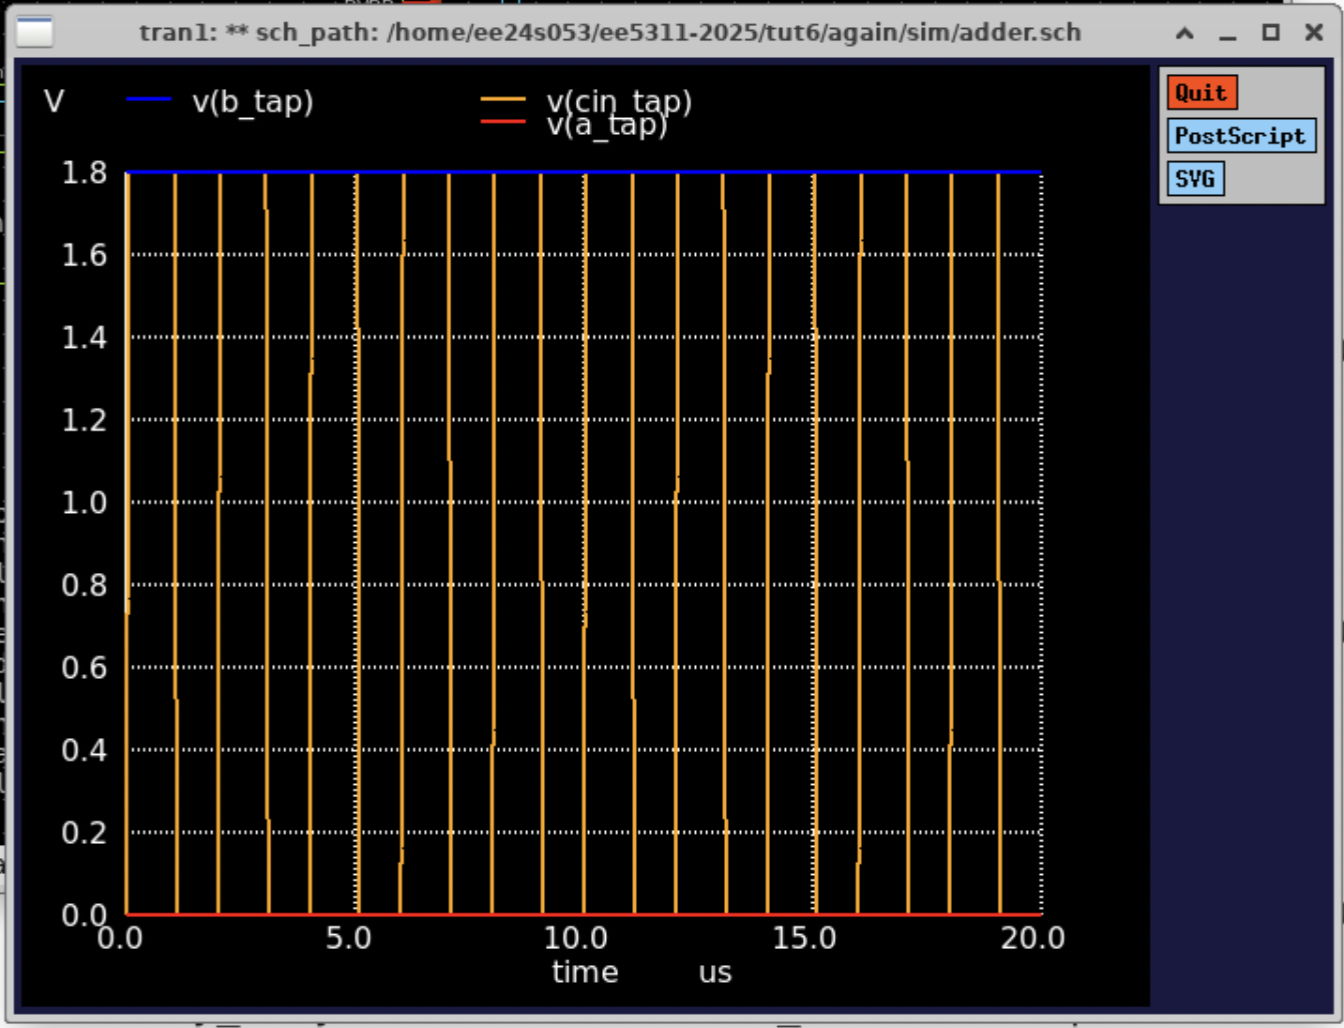
\includegraphics[width=0.47\linewidth]{tut6/reports/media/adder_inputs.png} &
     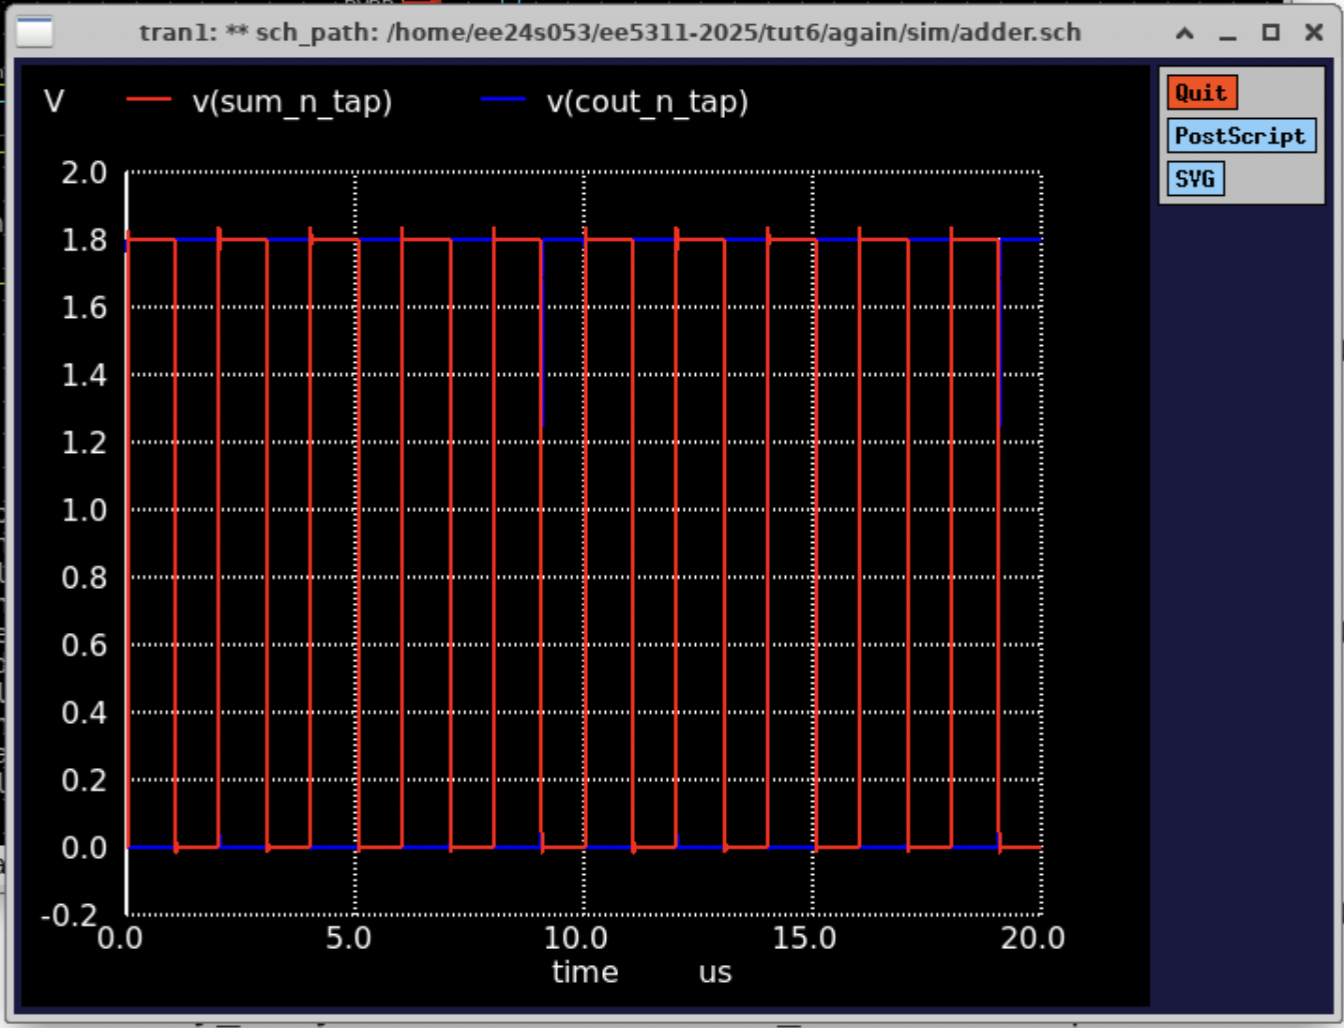
\includegraphics[width=0.47\linewidth]{tut6/reports/media/adder_outputs.png} \\
     Fig 5a: Input signals for the adder pre-layout & Fig 5b: Output signals for the adder pre-layout
\end{tabular}
\begin{tabular}{cc}
     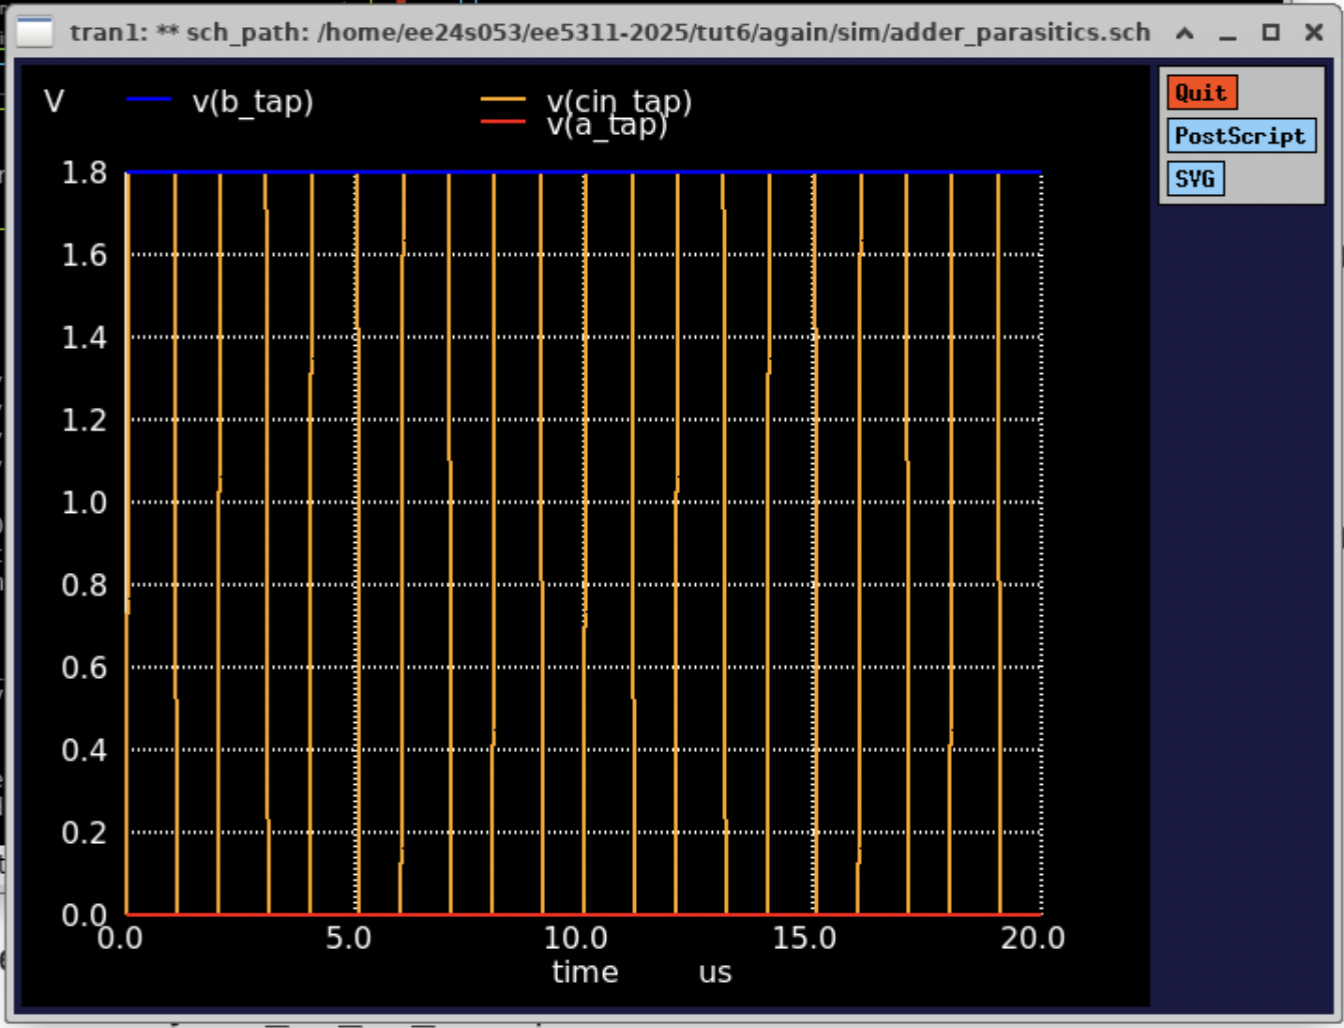
\includegraphics[width=0.47\linewidth]{tut6/reports/media/adder_parasitics_inputs.png} &
     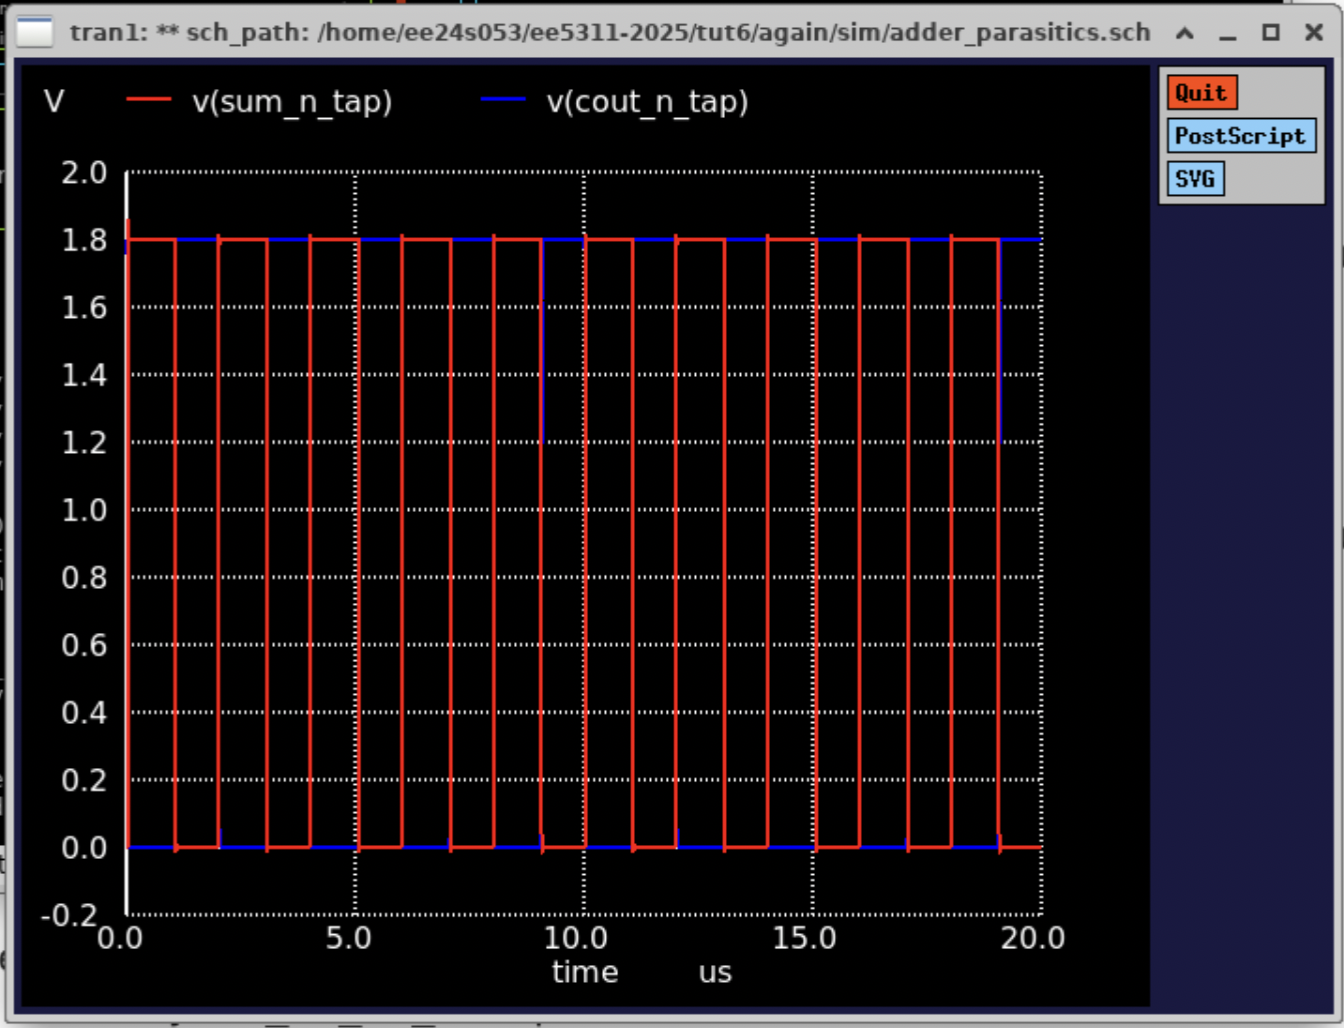
\includegraphics[width=0.47\linewidth]{tut6/reports/media/adder_parasitics_outputs.png} \\
     Fig 5c: Input signals for the adder post-layout & Fig 5d: Output signals for the adder post-layout
\end{tabular}
\end{center}
\noindent We obtain the following values for period and frequency without the layout parasitics.
\begin{verbatim}
tlh_carry           =  1.051850e-06 targ=  1.076850e-06 trig=  2.500000e-08
thl_carry           =  -1.050180e-06 targ=  2.481951e-08 trig=  1.075000e-06
carry delay: 8.35E-10
tlh_sum             =  -1.337493e-10 targ=  2.486625e-08 trig=  2.500000e-08
thl_sum             =  1.999316e-09 targ=  1.076999e-06 trig=  1.075000e-06
sum delay: 9.32786E-10
\end{verbatim}
\noindent We obtain the following values for period and frequency when we include the layout parasitics.
\begin{verbatim}
tlh_carry           =  1.051713e-06 targ=  1.076713e-06 trig=  2.500000e-08
thl_carry           =  -1.049846e-06 targ=  2.515425e-08 trig=  1.075000e-06
carry delay: 9.3E-10
tlh_sum             =  7.937398e-10 targ=  2.579374e-08 trig=  2.500000e-08
thl_sum             =  1.883455e-09 targ=  1.076883e-06 trig=  1.075000e-06
sum delay: 1.3386E-09
\end{verbatim}

\section{Declarations}
\begin{enumerate}
    \item I have publicly hosted this work on GitHub to help reproduce all of my results. The same can be accessed through the following \href{https://github.com/iamkarthikbk/ee5311-2025}{\underline{link}}.
\end{enumerate}

\end{document}
